\documentclass{article}

\usepackage{booktabs}
\usepackage{multirow}
\usepackage{amsmath}
\usepackage{hyperref}
\usepackage{overpic}
\usepackage{amssymb}
\usepackage{graphicx}

\usepackage[accepted]{dlaiml2026}

\dlaititlerunning{Search Beats Imitation in PTCG}

\begin{document}

\twocolumn[
\dlaititle{Search Beats Imitation: Neural-Guided Determinized MCTS\\for the Pok\'emon Trading Card Game}

\begin{center}\today\end{center}

\begin{dlaiauthorlist}
\dlaiauthor{Antonio Cordeiro}{}
\end{dlaiauthorlist}

\dlaicorrespondingauthor{Antonio Cordeiro}{antcor04@gmail.com}

\vskip 0.3in
]

\printAffiliationsAndNotice{}

\begin{abstract}
We build an agent for the Kaggle \emph{Pok\'emon TCG AI Battle Challenge}, a stochastic, imperfect-information card game with variable action sets. A 2.6M-parameter entity/option transformer is trained on 453k expert decisions with policy, value and opponent-hand (belief) heads; its value head is re-trained on self-play outcomes, and it guides a determinized Monte Carlo tree search on the exact game simulator. Under a rigorous protocol (held-out games, a fixed six-opponent gauntlet, 95\% Wilson intervals, SPRT), search raises the score against the gauntlet from 0.75 to 0.90 and the ladder rating from 650 (our previous system) to $\approx$790. A learned belief model predicts hidden cards better than counting (AUROC 0.75 vs 0.71) yet does not improve play: at our budgets one deep search tree beats averaging several shallow determinized trees.
\end{abstract}

% ------------------------------------------------------------------------------
\section{Introduction}
In the Pok\'emon TCG two players pilot 60-card decks; most information (hands, deck order, prize cards) is hidden, draws and coin flips are random, and the legal move set changes at every decision (play a card, attach, evolve, attack, pick targets, choose $k$ of $n$ cards). The Kaggle challenge provides a C++ simulator with a \emph{search} API that can step a game forward from any observation once the hidden cards are guessed, a ladder with a Gaussian skill rating, and a budget of $\approx$600\,s of thinking per best-of-3 match on 2 CPUs.

Our previous system stacked behavioural cloning, offline RL, PPO and weight averaging, but spent 6\,ms per move and reached only 250--650 on the ladder. Its local evaluation was invalid: in 350 games it rated the 500-ladder agent \emph{above} the 650-ladder one (score 0.32 for the latter). We therefore rebuilt the agent around (i) a simple network, (ii) search that actually uses the simulator and the time budget, and (iii) an evaluation protocol whose conclusions we can trust and check against the ladder. Code: \url{https://github.com/USER/ptcg-agent} (TODO).

% ------------------------------------------------------------------------------
\section{Related work}
AlphaGo/AlphaZero combine policy/value networks with PUCT tree search \cite{silver2016mastering,silver2018general}; expert iteration distils search back into the network \cite{anthony2017thinking}. For imperfect information, perfect-information Monte Carlo (PIMC) samples \emph{determinizations} of the hidden state and searches each \cite{long2010understanding}; information-set MCTS shares one tree across samples \cite{cowling2012information}. Entity/pointer transformers handle variable action sets in complex games \cite{vinyals2019grandmaster,vaswani2017attention}.

% ------------------------------------------------------------------------------
\section{Method}
\paragraph*{Representation and network.} Each observation becomes tokens: one global token (turn, prizes, deck/hand sizes, the decision type), two mean-pooled discard bags, up to 64 card tokens (Pok\'emon in play with HP, damage, energies; our hand; stadium; revealed cards) and up to 80 option tokens, one per legal move. An option token adds the embeddings of the card tokens it refers to (acting card, target), so the network scores moves by \emph{what they touch}; no card-specific rules are hand-coded. A 4-layer pre-norm transformer ($d{=}192$, 2.6M parameters) mixes all tokens. Heads: a policy over option tokens (plus a count head for $k$-of-$n$ choices), a value $V(s)\in[-1,1]$, and a belief head predicting, for every card id, whether it is in the opponent's hand.

\paragraph*{Training.} We parse the 3{,}000 highest-rated replays (453k decisions, split 90/5/5 \emph{by game}), pairing the observation at step $s$ with the action recorded at step $s{+}1$. Belief labels come for free: the replay stores the opponent's own view of its hand. The loss is cross-entropy on the chosen option(s) (losers' moves weighted 0.5) plus value MSE, count BCE and belief BCE (12 epochs, AdamW). With only 3k game outcomes the value head overfits (test Brier worse than a constant), so we fine-tune it on 8k games of policy self-play while anchoring the policy on replay batches. Optionally, expert iteration (ExIt) adds MCTS visit distributions from 1.6k search-vs-search games as policy targets.

\paragraph*{Search.} At each single-choice decision we sample $K$ worlds: our deck order and prizes uniformly from our unseen cards; the opponent's decklist as the library deck (120 decklists mined from replays and ladder games) most consistent with its visible cards; its hand either uniformly (count-based) or weighted by the belief head. In each world we run PUCT with network priors and value leaves on the simulator; forced moves and $k$-of-$n$ choices are played by the policy. Root visits are summed over worlds. A time manager spends $\min(c, (T_{\text{left}}-r)/q)$ seconds per decision, keeping a reserve of the 600\,s budget.

\paragraph*{Evaluation.} Offline metrics on held-out test games. Online: a fixed \emph{gauntlet} of six opponents (our two previous Kaggle agents with their decks, and our imitation policy piloting four meta decks), seat-balanced, with a simulated Kaggle time budget; we report scores with 95\% Wilson intervals, use paired head-to-head matches for ablations and an SPRT ($H_0$: +0, $H_1$: +30 Elo) to gate submissions.

% ------------------------------------------------------------------------------
\section{Results}
\begin{table}[t]
\caption{Top: offline results on held-out games. Bottom: online ablations (score of A vs B, 95\% CI).}
\label{tab:results}
\begin{center}
\begin{small}
\begin{tabular}{@{}lr@{}}
\toprule
Policy top-1 (uniform-legal baseline) & 70.0\% (21.7\%) \\
\quad main phase, $\geq$5 options & 60.7\% (11.6\%) \\
Value Brier: replay-only / +self-play (const.) & .254 / .226 (.249) \\
Belief AUROC: learned / count w/ true list & .752 / .711 \\
\midrule
MCTS-64 vs own policy (200 games) & .59 [.52, .66] \\
learned vs count-based hand sampling (400) & .48 [.43, .53] \\
4 worlds vs 1 world, equal sims (300) & .39 [.34, .45] \\
deployed: 1 vs 4 worlds (400) & .57 [.52, .61] \\
ExIt-2 + MCTS vs base + MCTS (300) & .57 [.51, .62] \\
ExIt-3 + MCTS vs ExIt-2 + MCTS (300) & .50 [.45, .56] \\
searching $k$-of-$n$ choices vs policy (400) & .48 [.43, .53] \\
\bottomrule
\end{tabular}
\end{small}
\end{center}
\vspace{-0.5cm}
\end{table}

\begin{figure}[t]
\centering
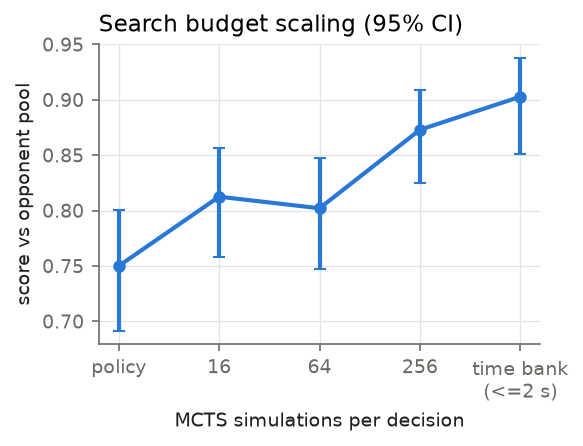
\includegraphics[width=0.85\linewidth]{figures/search_scaling.png}
\vspace{-0.3cm}
\caption{Score against the six-opponent gauntlet (Crustle deck, 180--240 games per point, 95\% CI) as a function of search budget; ``time bank'' is the deployed agent (up to 2\,s per decision).}
\label{fig:scaling}
\vspace{-0.4cm}
\end{figure}

\paragraph*{Offline.} The policy predicts expert moves far above chance (Tab.~\ref{tab:results}); two seeds agree within 0.3 points. Self-play fixes the overfit value head. The belief head beats a count-based baseline that is even given the opponent's true decklist, without access to the decklist, presumably by learning from the public game state which cards players tend to hold.

\paragraph*{Deck choice.} Piloted by our policy, the deck that dominates top-rated replays (Dragapult, 57\% win rate there) scores only 0.49 against the gauntlet, while a Kangaskhan/Crustle deck scores 0.73 (240 games each): the best deck for an agent depends on the agent.

\paragraph*{Search.} Search is the main source of strength (Fig.~\ref{fig:scaling}): 0.75 for the raw policy, 0.87 at 256 simulations, 0.90 for the deployed agent (0.93 against a reconstruction of our previous best Kaggle agent), reproduced on a second seed. Surprisingly, the learned belief gives no measurable gain when used to sample hands, and splitting a fixed budget over four determinizations is \emph{worse} than one deep tree ($-75$ Elo): at these depths the tree rarely reaches situations where the opponent's exact hand matters. ExIt with 64-simulation targets does not change the raw policy (0.50) but makes the search stronger (+49 Elo), while ExIt with noisy 16-simulation targets did not help and a third round brought no further gain (0.50). Extending search to $k$-of-$n$ card choices did not help either (0.48).

\paragraph*{Ladder.} Our previous agents sit at 650 and 500. The new agent rated $\approx$737 (4 worlds) and $\approx$768 (1 world) after 10 hours; adding the ExIt-2 network, a 3\,s cap and a 120-deck opponent library reached $\approx$794 after 4 hours (score 0.65 over 52 matches), our best. Unlike the old protocol, the local ranking (1 world $>$ 4 worlds) matches the ladder.

% ------------------------------------------------------------------------------
\section{Discussion and conclusions}
A small imitation network is a good prior, but the gains come from looking ahead with the real game engine. Better hidden-information modelling helps prediction but not play at our search depth, a negative result we confirmed with two budgets and an ablation on the number of worlds. Limitations: four of six gauntlet opponents share our network, ladder ratings are still converging, and expert iteration plateaued after two useful rounds at our compute.

% ------------------------------------------------------------------------------
\section{Statement on the use of AI}\label{sec:ai}
I used an AI assistant (Claude, Anthropic) extensively throughout the project, as a pair programmer and research assistant. It helped review the previous code base and its failure modes, propose the experimental plan, write most of the new code (replay parser, tokeniser, model and training scripts, self-play, MCTS, evaluation and statistics, submission packaging), launch and monitor experiments on my machine through a job runner, analyse results, produce the plots, and draft this report. I chose the direction of the project, reviewed the code and results, ran the Kaggle submissions, and checked that every number in this report comes from the logged experiments (\texttt{RESULTS.md} in the repository); I take full responsibility for the content and can explain all parts of it.

\bibliography{references.bib}
\bibliographystyle{dlaiml2026}

\clearpage
\appendix
\section*{Appendix: additional results}
\begin{figure}[h]
\centering
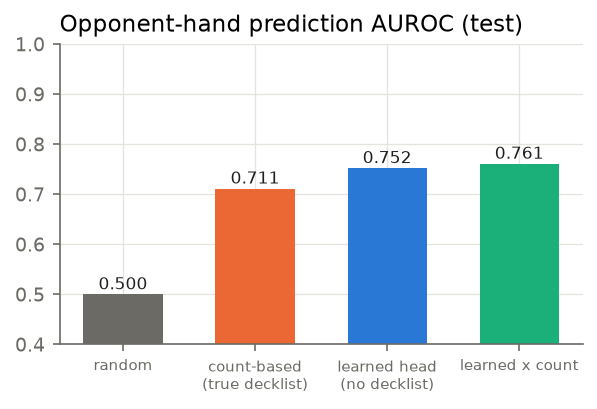
\includegraphics[width=0.48\linewidth]{figures/belief_auroc.png}\hfill
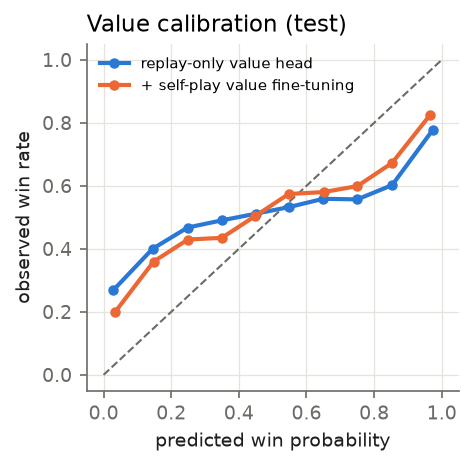
\includegraphics[width=0.40\linewidth]{figures/value_calibration.png}
\caption{Left: opponent-hand prediction AUROC on held-out games. Right: value calibration on held-out replay games before and after self-play fine-tuning (Brier .254 $\rightarrow$ .226).}
\end{figure}
\begin{figure}[h]
\centering
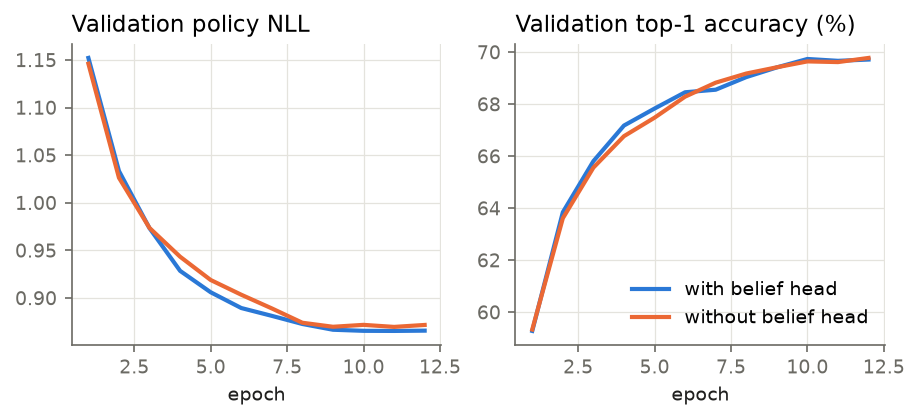
\includegraphics[width=0.95\linewidth]{figures/training_curves.png}
\caption{Validation curves with and without the auxiliary belief head (no effect on the policy).}
\end{figure}
\begin{table}[h]
\caption{Additional ablations (Crustle mirror, MCTS-64, 1 world; score of A vs B, 95\% CI).}
\begin{center}\begin{small}
\begin{tabular}{@{}lr@{}}
\toprule
$c_{\text{puct}}=0.7$ vs $1.25$ (240 games) & .51 [.45, .58] \\
$c_{\text{puct}}=2.5$ vs $1.25$ (240 games) & .43 [.37, .49] \\
deployed: 3\,s cap + 120-deck library vs 2\,s, 8 decks (160) & .54 [.46, .61] \\
\bottomrule
\end{tabular}
\end{small}\end{center}
\end{table}
\begin{table}[h]
\caption{Deck selection: our policy piloting each deck against the gauntlet (240 games each).}
\begin{center}\begin{small}
\begin{tabular}{@{}lr@{}}
\toprule
Mega Kangaskhan ex / Crustle & .73 [.67, .78] \\
Teal Mask Ogerpon ex & .65 [.59, .71] \\
Hydrapple ex & .64 [.58, .70] \\
Marnie's Grimmsnarl ex & .59 [.53, .65] \\
Dragapult ex & .49 [.43, .56] \\
Lillie's Clefairy ex & .28 [.23, .34] \\
\bottomrule
\end{tabular}
\end{small}\end{center}
\end{table}

\end{document}
